\documentclass{article}
\usepackage[utf8]{inputenc}
\usepackage{amsmath}
\usepackage{natbib}
\usepackage{graphicx}
\usepackage{astrojournals} % Necesario para nombres de revistas en luis-ref.bib
\usepackage[spanish, es-minimal]{babel}
\bibliographystyle{apj}
\newcommand\U[1]{\ensuremath{\mathrm{#1}}}
\newcommand\K{\U{K}}
\newcommand\cm{\U{cm}}
\newcommand\AU{\U{AU}}
\newcommand\g{\U{g}}
\newcommand\msolagno{M_\odot\,\U{yr^{-1}}}

\newcommand\acre{\ensuremath{_{\mathrm{acre}}}}
\newcommand\eff{\ensuremath{_{\mathrm{eff}}}}
\newcommand\Ext{\ensuremath{_{\mathrm{Ext}}}}
\newcommand\Int{\ensuremath{_{\mathrm{Int}}}}
\newcommand\ha{\ensuremath{\mathrm{H}\alpha}}
\newcommand\nii{\ensuremath{\mathrm{[N\,II]}}}
\title{Seminario de investigación II:\\ Stationary bowshock arcs in the Orion Nebula}

\author{
  Alumno: Luis Angel Gutiérrez Soto\\
  Tutor: Dr. William Henney
}

\begin{document}
\maketitle

\section{Motivación}
\label{sec:motivacion}

En los últimos años se han identificado un número considerable de Objetos LL en la Nebulosa de Orión, los cuales son estrellas T Tauri que se caracterizan por presentar un arco de emisión circumstellar.
El prototipo de estos objetos es la estrella LL~Ori cuya emisión circunestelar fue descubierto hace 36 años \citep{Gull:1979a}. 
No obstante varios de estos objetos con estas características fueron identificadas por Bally, los cuales ha mencionado y enlistado en varios de sus artículos \citep{Bally:2000a, Bally:2001a, Bally:2006a}, pero hay que tener en cuenta que no existe una lista completa de todos los objetos LL que se han encontrado en dicha región, es así que el principal objetivo de este trabajo es crear un catálogo muy completo de todos los arcos de choque de proa estacionarias  que hasta el momento se han identificado.\\

Como ya se ha mencionado, a los objetos LL se les asocia un choque estacionario, debido a que el flujo de ``Champagne'' proveniente del trapecio, que entre otras cosas es ligeramente supersónico (\(M\simeq2\)) choca con un obstáculo, que en este caso es un flujo también supersónico asociado a una estrella T Tauri, originando desde luego un arco hyperbólico, no obstante la zona chocada es muy radiativa proporcionando un arco de emisión brillante el cual resulta ser muy visible, la naturaleza del obstáculo; es posible que se deba a un Proplyd radiactivo o el viento de una estrella T Tauri.\\ 


Otro de los propósitos de este trabajo es realizar un estudio de las características físicas de los choques, en este sentido se prentende estudiar parámetros físicos como el brillo superficial, el cúal se podría medir utilizando las observaciones del HST con las cámaras  WFPC2, ACS y WFC3, y en este orden de ideas analizar las imágenes de \ha{} y \nii{} en las diferentes zonas del choque, esto es; la zona pos-choque, en la cáscara chocada y en la parte interna del mismo. Esto va a hacer muy importante porque una vez medido el brillo y junto al radio de curvatura \(R_{c}\), es factible calcular la densidad \(n\) y con esta se puede  estimar la tasa de pérdida de masa \(\dot{M}\) de los objetos en cuestión, sin olvidar que hay  que considerar otros parámetros como la temperatura y la emisividad. En última instancia estas serían las razones por las cuales se considera este estudio. 

\section{Descripción de los datos}
\label{sec:descripcion}

\subsection{Cámaras y telescopio}
\label{sec:camara}

Para este estudio se usan observaciones del telescopio espacial HST, debido a que este brinda las posibilidades de obtener imágenes concretas de la Nebulosa de Orión, permitiendo en este sentido examinar sus componentes estelares, para generar estas imágenes se usaron las cámaras  WFPC2 y ACS con el objetivo de obtener observaciones en emisiones de \ha{}.\\

Hemos trabajado principalmente con las imágenes de \citet{Bally:2006a}, las cuales vienen de la cámara ACS, está a su vez está basada en un mosaico de dos detectores CCD de \(2048 \times 4096\) pixeles, la óptica del instrumento ofrece una escala espacial de \(\sim\) 50 mas/pixel, correspondiendo a un campo de visión de aproximadamente \(100'' \times 200'' \) \citep{Robberto:2013a}. Es así que se usan filtros de banda ancha, esto es de aproximadamente \(50 \text{Å}\). La importancia de utilizar las imágenes de Bally radica en que la señal a ruido es muy buena, debido a que tiene tiempos más largos de exposición. Esta cámara contiene el filtro f658n, el cual permite ver las emisiones de \ha{} y \nii{}. Para nuestro trabajo vamos a utilizar estas imágenes para trazar los arcos radiativos de los choques, este filtro es importante porque permite mapear el material que rodea a las estrellas con la más alta resolución posible y de la misma forma permite discriminar fuentes extendidas de emisión. Sin embargo la desventaja de utilizar estas observaciones es que no tiene una cobertura completa de la Nebulosa de Orión y además admite las líneas de \nii{}. Por otro lado toda la región que se logra mapear está divida en 26 campos, de las cuales nuestros objetos se encuentran repartidos en los campos: 01, 02, 06, 07, 08, 09, 14, 16, 17 y 24.\\

De la misma manera se han utilizado aunque en menor grado las observaciones de Robberto, las cuales utilizan la cámara WFPC2 para tomar sus datos, este tiene la ventaja de que además de cubrir toda la Nebulosa de Orión tiene el filtro f656n, el cual es un filtro de \ha{} que no deja pasar las líneas de  \nii{}.\\ 

En resumidas cuentas el propósito de utilizar estos dos filtros (f656n y f658n), consiste en que así es posible separar las emisiones de \ha{} y \nii{}.       

\section{Metodología}
\label{sec:metodo}

\subsection{Arcos}
\label{sec:arcos}

Con el objetivo de obtener algunos paŕametros, tales como el  radio de curvatura \(R_{c}\), la distancia de la estrella a la cáscara chocada \(R_{0}\) y la distancia \(D\) de la estrella al trapecio, de tal manera  que permitan entender la naturaleza de los choques estacionarios.Para tratar las imágenes de Bally se utiliza el programa ``ds9'' y  una vez identificados todos los Objetos LL en los diferentes campos, se trazan las formas de los arcos, para ello se establecen los límites de la cáscara chocada, valiendonos de los herramientas de dicho pograma, en este sentido para establecer las coordenadas de la estrella se utiliza un círculo, para el borde externo de la cáscara se trazan las coordenadas del mismo limitándolas con ``x'' y para el borde interno se establecen los puntos que lo forman usando ``+'' como se observa en la figura \ref{fig:LL1-Bally}, es así que de esta manera se obtienen los  arcos hiperbólicos.

\begin{figure}
  \centering
  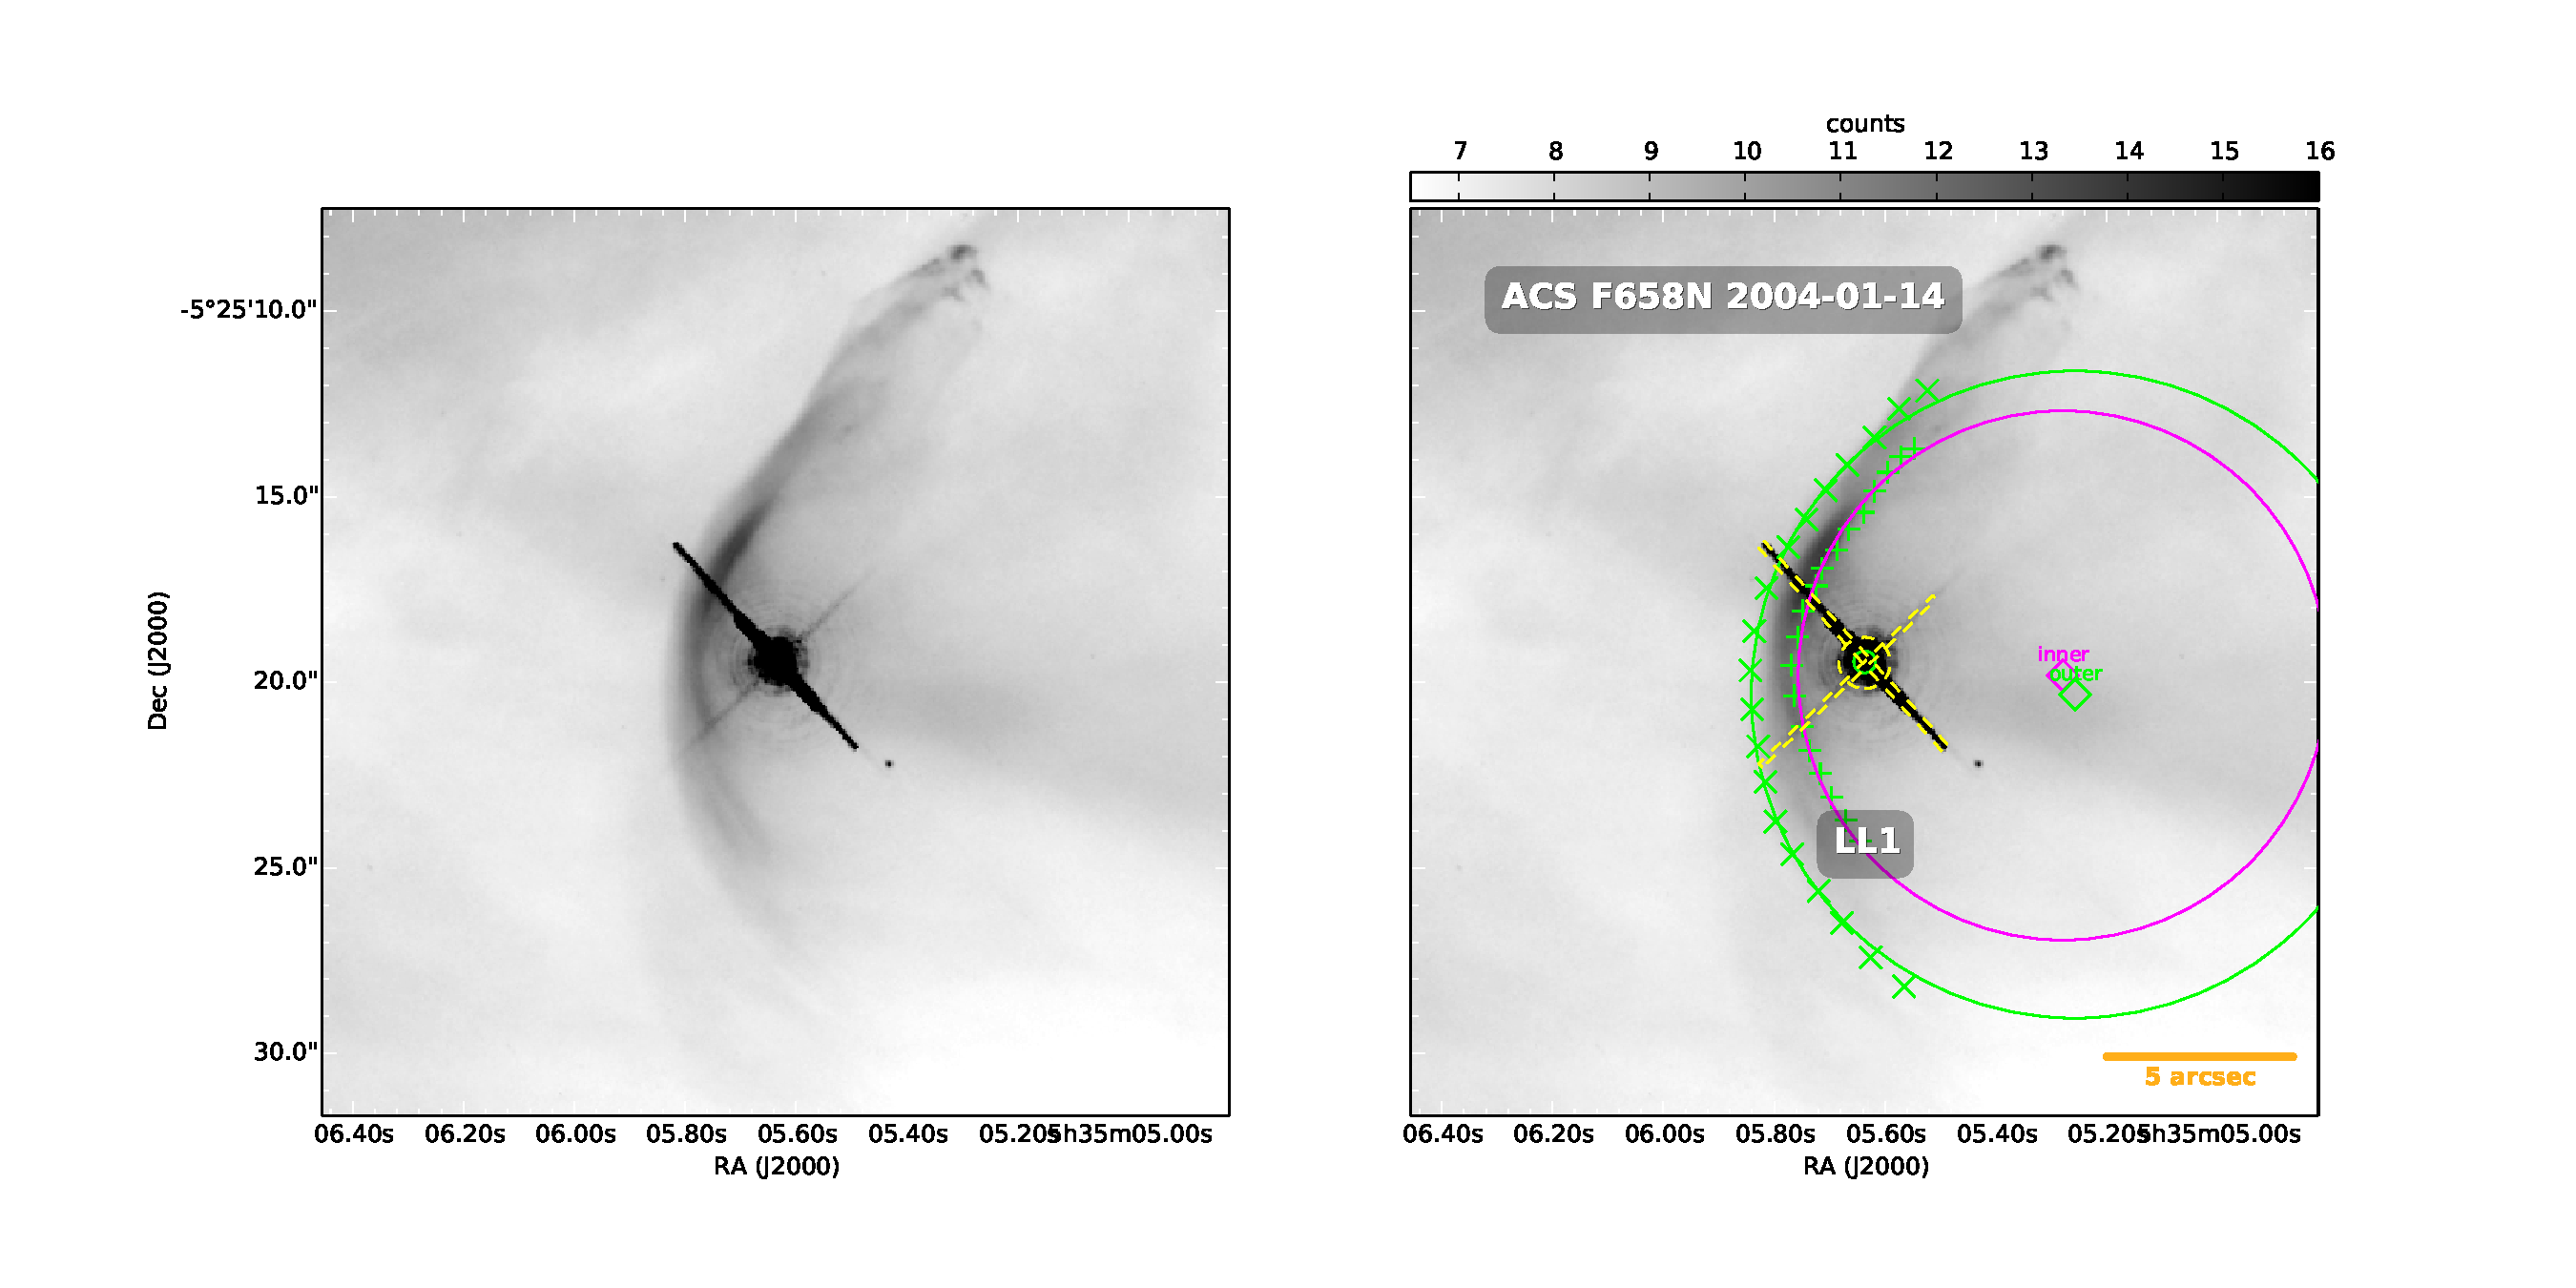
\includegraphics[width=\linewidth]{j8oc01010_wcs/LL1-Bally_01-images.pdf}
  \caption{Forma de los choques (LL1)}
  \label{fig:LL1-Bally}
\end{figure}

\subsection{Radio de curvatura}
\label{sec:curvatura}

Una vez trazada la forma de los arcos, se ajustan círculos a los puntos que forman tanto el borden externo como el interno del choque, logrando con esto determinar el radio de curvatura (\(R_{c}\)) de nuestros objetos, no obstante es importante señalar que el el centro de los círculos no va a coincidir con la posición del Proplyds, es más la distancia entre estos dos puntos (estrella y el centro de círculo)  va a variar dependiendo de la posiciones de los puntos que se han trazado para determinar la zona chocada. La figura \ref{fig:ajuste-circulo} nos muestra ajustes de círculos para el borde externo y el borde interno de LL1 y ahí claramente se observa la discrepancia entre la posición del objeto en cuestión y el centro de los círculos.\\

\begin{figure}
  \centering
  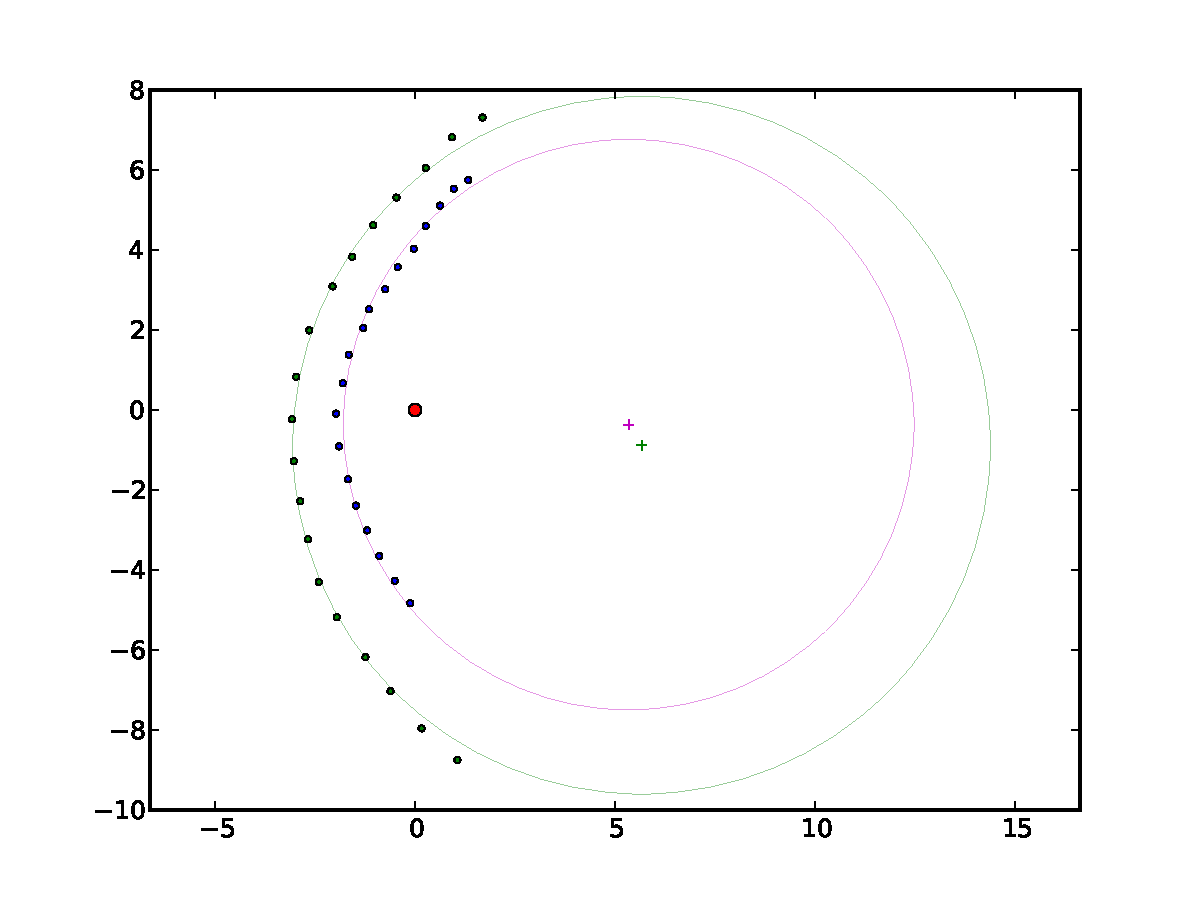
\includegraphics[width=.8\linewidth]{j8oc01010_wcs/LL1-arcfits.pdf}
  \caption{Ajustes de los círculos en los bordes del choque para LL1}
  \label{fig:ajuste-circulo}
\end{figure}

\subsection{Brillo superficial}
\label{sec:brillo}

Después de haber trazado los arcos  hemos establecido el brillo superficial \(S_{H\alpha}\) en la zona chocada, utilizando nuevamente las herramientas de ``SAOImage DS9'', es decir podemos conocer el brillo en cualquier punto de interés, no obstante como ya habíamos modelado la forma de los choques estacionarios, entonces pudimos medir el brillo en diferentes puntos de la zona chocada, es decir se midió este parámetro a diferentes ángulos con respecto al eje de simetría (dirección en la que llegan los fotones de la estrella masiva), pero no sólo basta medir el brillo en el gas chocado, es así que hemos medido este en la región interna y de la misma manera en el fondo, es decir la parte exterior del choque. Sin embargo como sólo se puede obtener el brillo en un punto en partícular, hemos obtenido el brillo en muchos puntos y a partir de ahí hemos realizado estadística, para estimar el brillo en la cáscara chocada y en el fondo.       
 
\section{Análisis teórico}
\label{sec:teoria}

\subsection{Estimación de la presión de la cáscara chocada}
\label{sec:presion}

\noindent En esta parte del trabajo estimemos el producto \(\dot{M}v\), consideremos que la presión del ambiente, es igual a la presión térmica en el gas chocado y esto a su vez es igual a la presión interna.\\

\begin{figure}
  \centering
   \includegraphics[width=.8\linewidth]{Foto0021.pdf}
  \caption{Los arcos de los Objetos LL son producidos cuando un flujo de gas ionizado choca con un obstáculo que pude ser; un  Proplyd radiactivo con densidad \(n \sim 10^{3}-10^{4}\cm^{-3}\) y velocidad \(v\sim 20-40 \text{km}/\text{s}\) o el  viento de una estrella T Tauri con densidad \(n \sim 100 \cm^{-3}\) y velocidad \(v\sim 100 \text{km}/\text{s}\), que puede o no ser radiactivo.}
  \label{fig:presion-cascara}
\end{figure}

\noindent También se supone que:
\begin{enumerate}
\item  Estado estacionario (tiempo dinámico \(\textless\) tiempo evolutivo)
\item  No hay aceleración ni gravedad.
\item  Para las siguientes componentes hay que tener en cuenta:
\end{enumerate}

\begin{itemize}
\item  Viento: domina presión hidrodinámica.
\end{itemize}
\begin{itemize}
\item  Cásacara chocada: domina presión térmica.
\end{itemize}

 De donde 

\begin{equation}
  \label{eq:igualda-presion}
  P_{\text{int}}=P_{\text{térmica}}=P_{\text{ind}}(\text{interna})
\end{equation}

\noindent ahora, la región interna experimenta una pérdida de masa puesto que en esa zona existen vientos, por tanto

\begin{equation}
  \label{eq:perdida-masa}
  \dot{M}=4\pi \rho v R^{2}
\end{equation}

\noindent el viento estelar tiene por presión,

\begin{equation}
  \label{eq:presion-viento}
  P=\rho v^{2}
\end{equation}

\noindent y en este sentido tendremos que la presión interna está dada por  

\begin{equation}
  \label{eq:presin-interna}
  P_{\text{int}}=\frac{\dot{M} v}{4 \pi R^{2}}. 
\end{equation}

 Por otro lado la presión en la cáscara sería;

\begin{equation}
  \label{eq:presion-cascara}
  P_{c}=2 n k T 
\end{equation}

\noindent donde \(n\) es la densidad numérica de núcleos de H y \(T\) es la temperatuta, para la cual se podría considerar \(\text{T} \simeq 10^{4}\K\), no obstante también se  estimaría T a partir de: i) cocientes de líneas colisionales, [OIII] 4363/5007, [NII] 5755/6554. ii) Ensanchamiento comparativo entre H y N. iii) Cociente de línea/ continuo, esto es Radio: RR/Brems y azul/uv (Balmer jump).\\

 Ahora de ~(\ref{eq:igualda-presion}),  ~(\ref{eq:presin-interna}) y  ~(\ref{eq:presion-cascara}) , obtendremos una expresión de la tasa de pérdida de masa dada por:

\begin{equation}
  \label{eq:perdida-masa}
  \dot{M}v = 8 \pi n kR T. 
\end{equation}

 Para estimar \(n\) implementamos el hecho. Como se dijo anteriormente de las observaciones podemos obtener \(S_{\ha}\) y dado que si suponemos que no hay obsorción entonces 

\begin{equation}
  \label{eq:brillo}
  S_{\ha} = \int \eta_{\ha} d\zeta \simeq \eta_{\ha} \Delta \zeta
\end{equation}

\noindent en la que \(\eta_{\ha}\) es la emisividad y \(\Delta \zeta\) es el cámino de la línea de visión. Si la tasa de recombinaciones por volumen que producen \ha{}  es 
\begin{equation}
  \label{eq:recombinaciones}
  \alpha_{\ha} n_{e}n_{H^{+}}=n(H^0_{\text{n}=3})A_{32}
\end{equation}

\noindent dado que el coeficiente de emisión es

\begin{equation*}
 \eta_{\ha} = n(H^0_{\text{n}=3})A_{32} \left(\frac{hc}{\lambda_{32}}\right) \frac{1}{4\pi}
\end{equation*}

\noindent si se sustituye esta última expresión en ~(\ref{eq:recombinaciones}) y teniendo en cuenta que \(n_{e}\simeq n_{H} \simeq n\) obtenemos que

\begin{equation*}
 \eta_{\ha} =  \frac{\alpha_{\ha}n^{2}}{4\pi} \left(\frac{hc}{\lambda_{32}}\right)  
\end{equation*}

\noindent así que usando la ec. ~(\ref{eq:brillo}) se concluye que,

\begin{equation}
  \label{eq:densidad}
  n^{2}=\frac{S_{\ha} 4 \pi}{\alpha_{\ha} E_{32} \Delta \zeta}
\end{equation}

\noindent donde \( E_{32}\) es la energía de los fotones en la emisión de \ha{}  y \(\alpha_{\ha}=1.27\times 10^{-13}\cm^{3} \text{s}^{-1} \) es el coeficiente recombinación efectiva.\\

\subsection{Estimación de \(\Delta \zeta\)}
\label{sec:delta}

A partir del radio de curvatura \(R_{c}\) y del ancho de la zona chocada \(h\) podemos determinar \(\Delta \zeta\) (ver figura~\ref{fig:geometria}), suponiendo simetría silíndrica y el eje de simetría en el plano del cielo (xy).\\

\begin{figure}
  \centering
  \includegraphics[width=.8\linewidth, trim=30 150 30 150, clip]{Foto0081.pdf}
  \caption{Geometría de la cáscara chocada.}
  \label{fig:geometria}
\end{figure}

Entonces como la geometría de la cáscara en xz es igual e xy.  así que para \(h \gg R_{c}\) tendremos que,

\begin{equation}
  \label{eq:vision}
  \Delta \zeta = 2(R_{c}h)^{1/2}
\end{equation}

\section{ Resultados preliminares}
\label{sec:resultado}

En este trabajo hemos agregado a nuestra lista 72 objetos con sus respectivos choques de donde hemos podido substraer la zona chocada, como anteriormente hemos dicho esto nos ha permitido caracterizar las estrellas objetos de estudios, en la medida en que hemos podido determinar \(R_{c}\) y \(R_{0}\) tanto de los bordes internos y externos, parámetros importante para especificar tópicos astrofísicos de los mismos.\\


\begin{figure}[htp]
\centering
\begin{tabular}{l l}
(a) & \\
 & 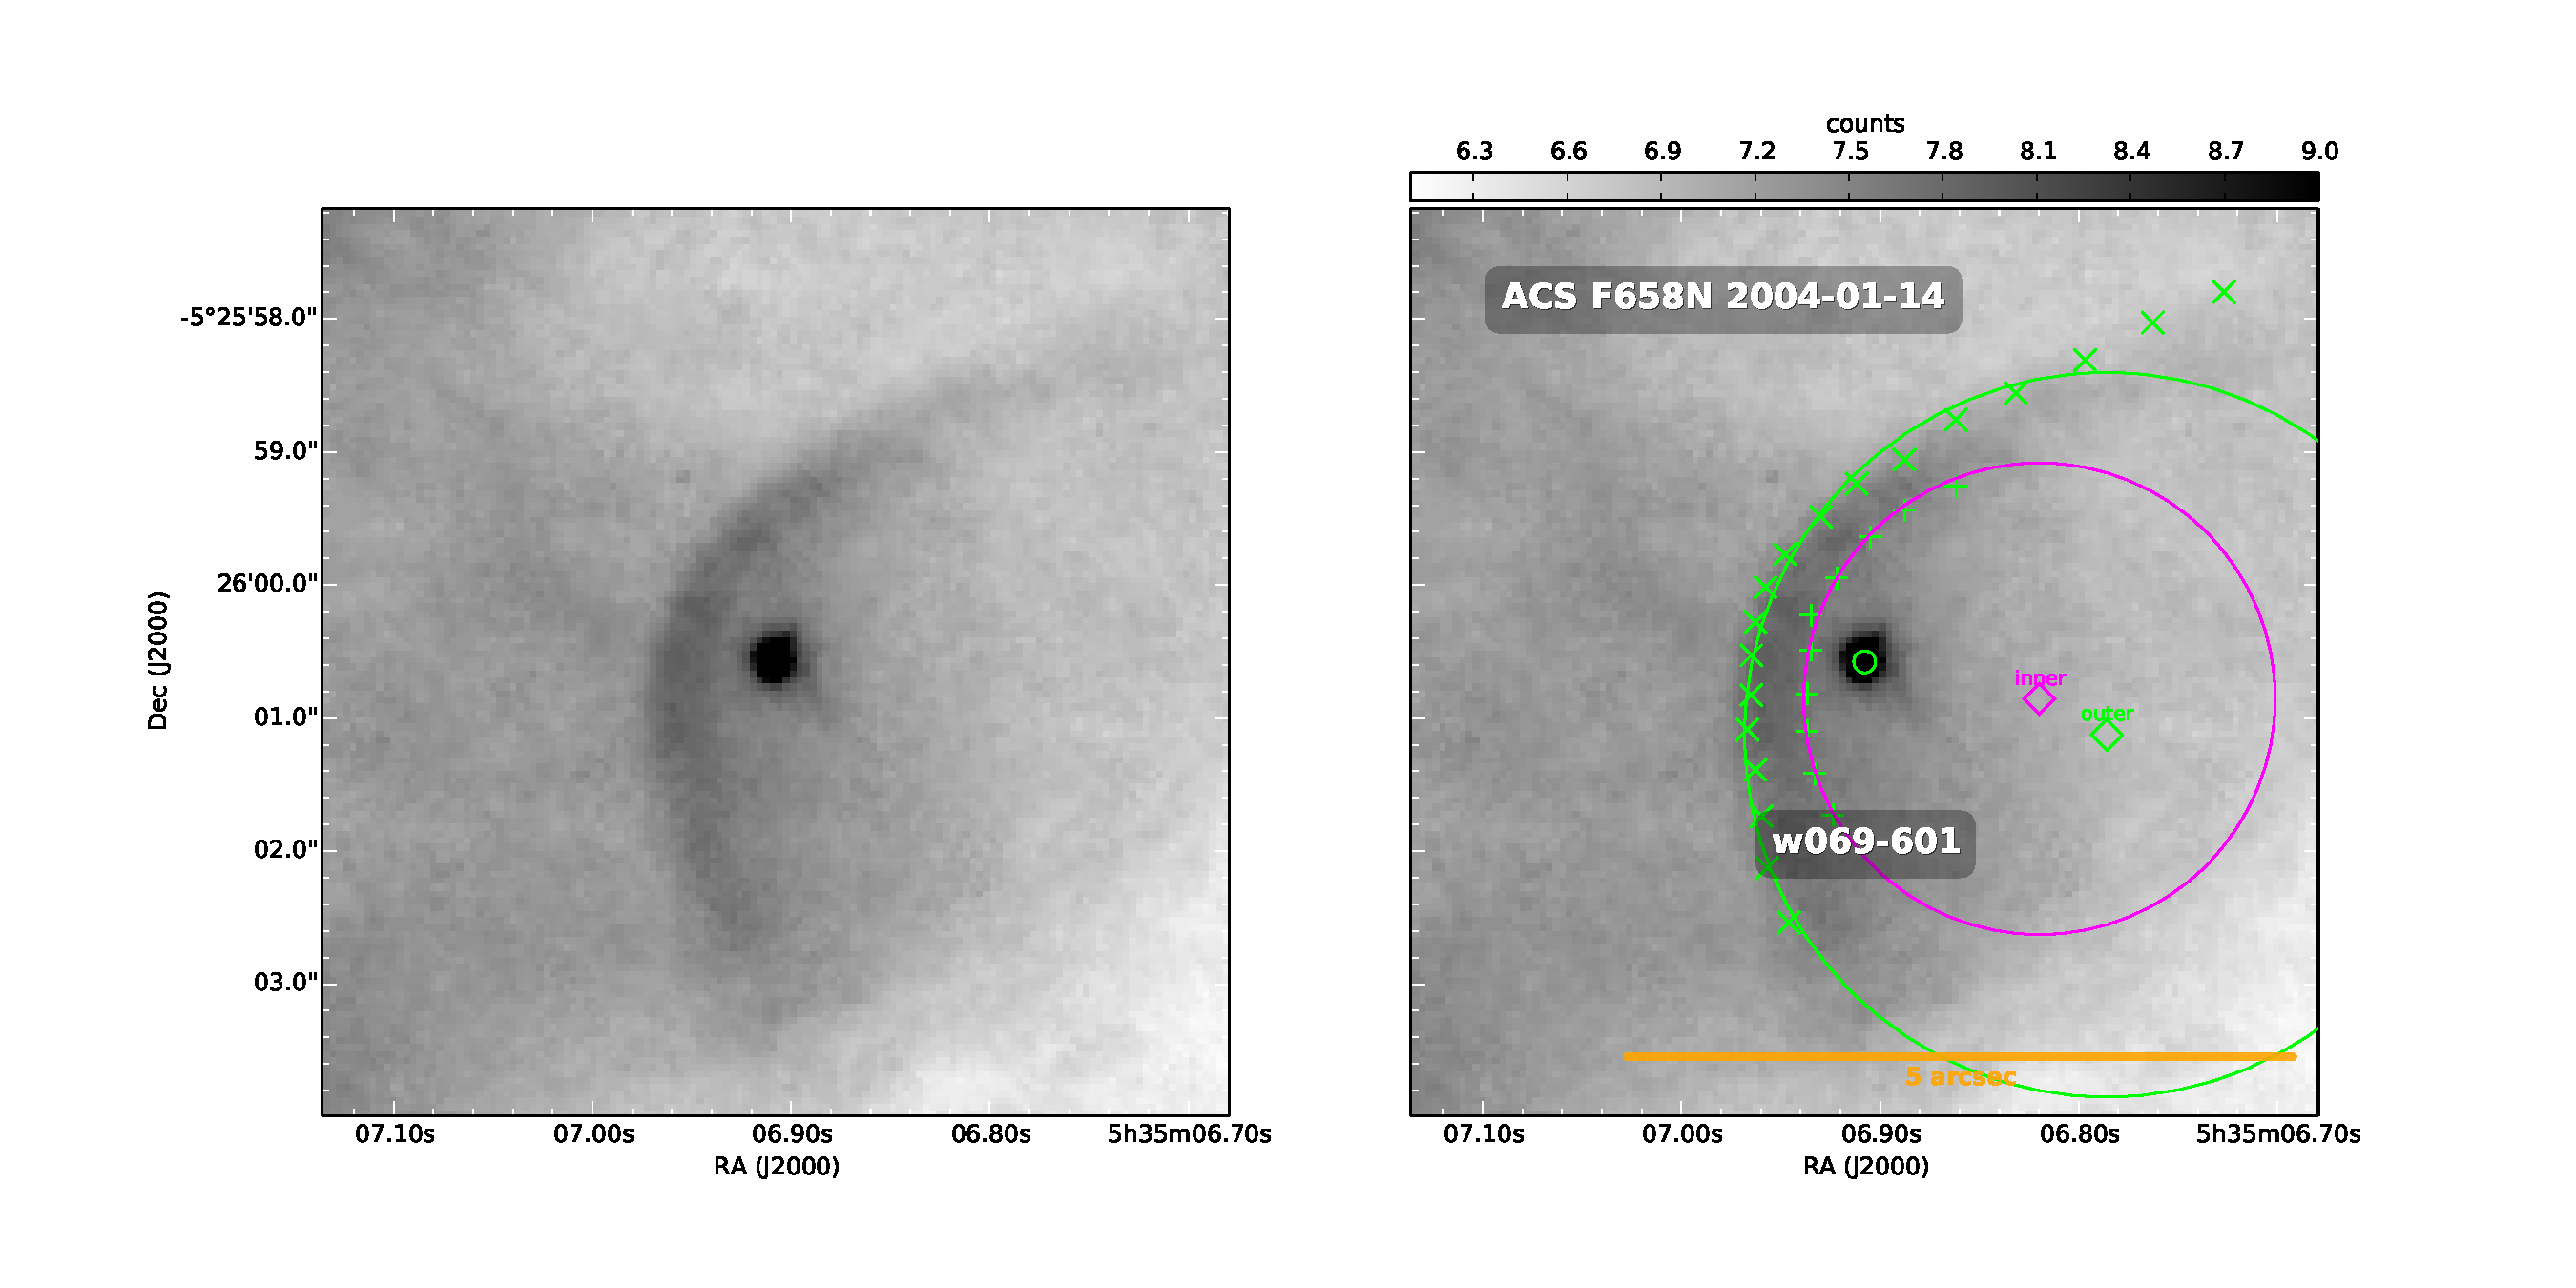
\includegraphics[width=0.95\linewidth, trim=60 20 60 60, clip]{./j8oc01010_wcs/w069-601-Bally_01-images.pdf}
\\
& \\[2\baselineskip]
(b) & \\
& 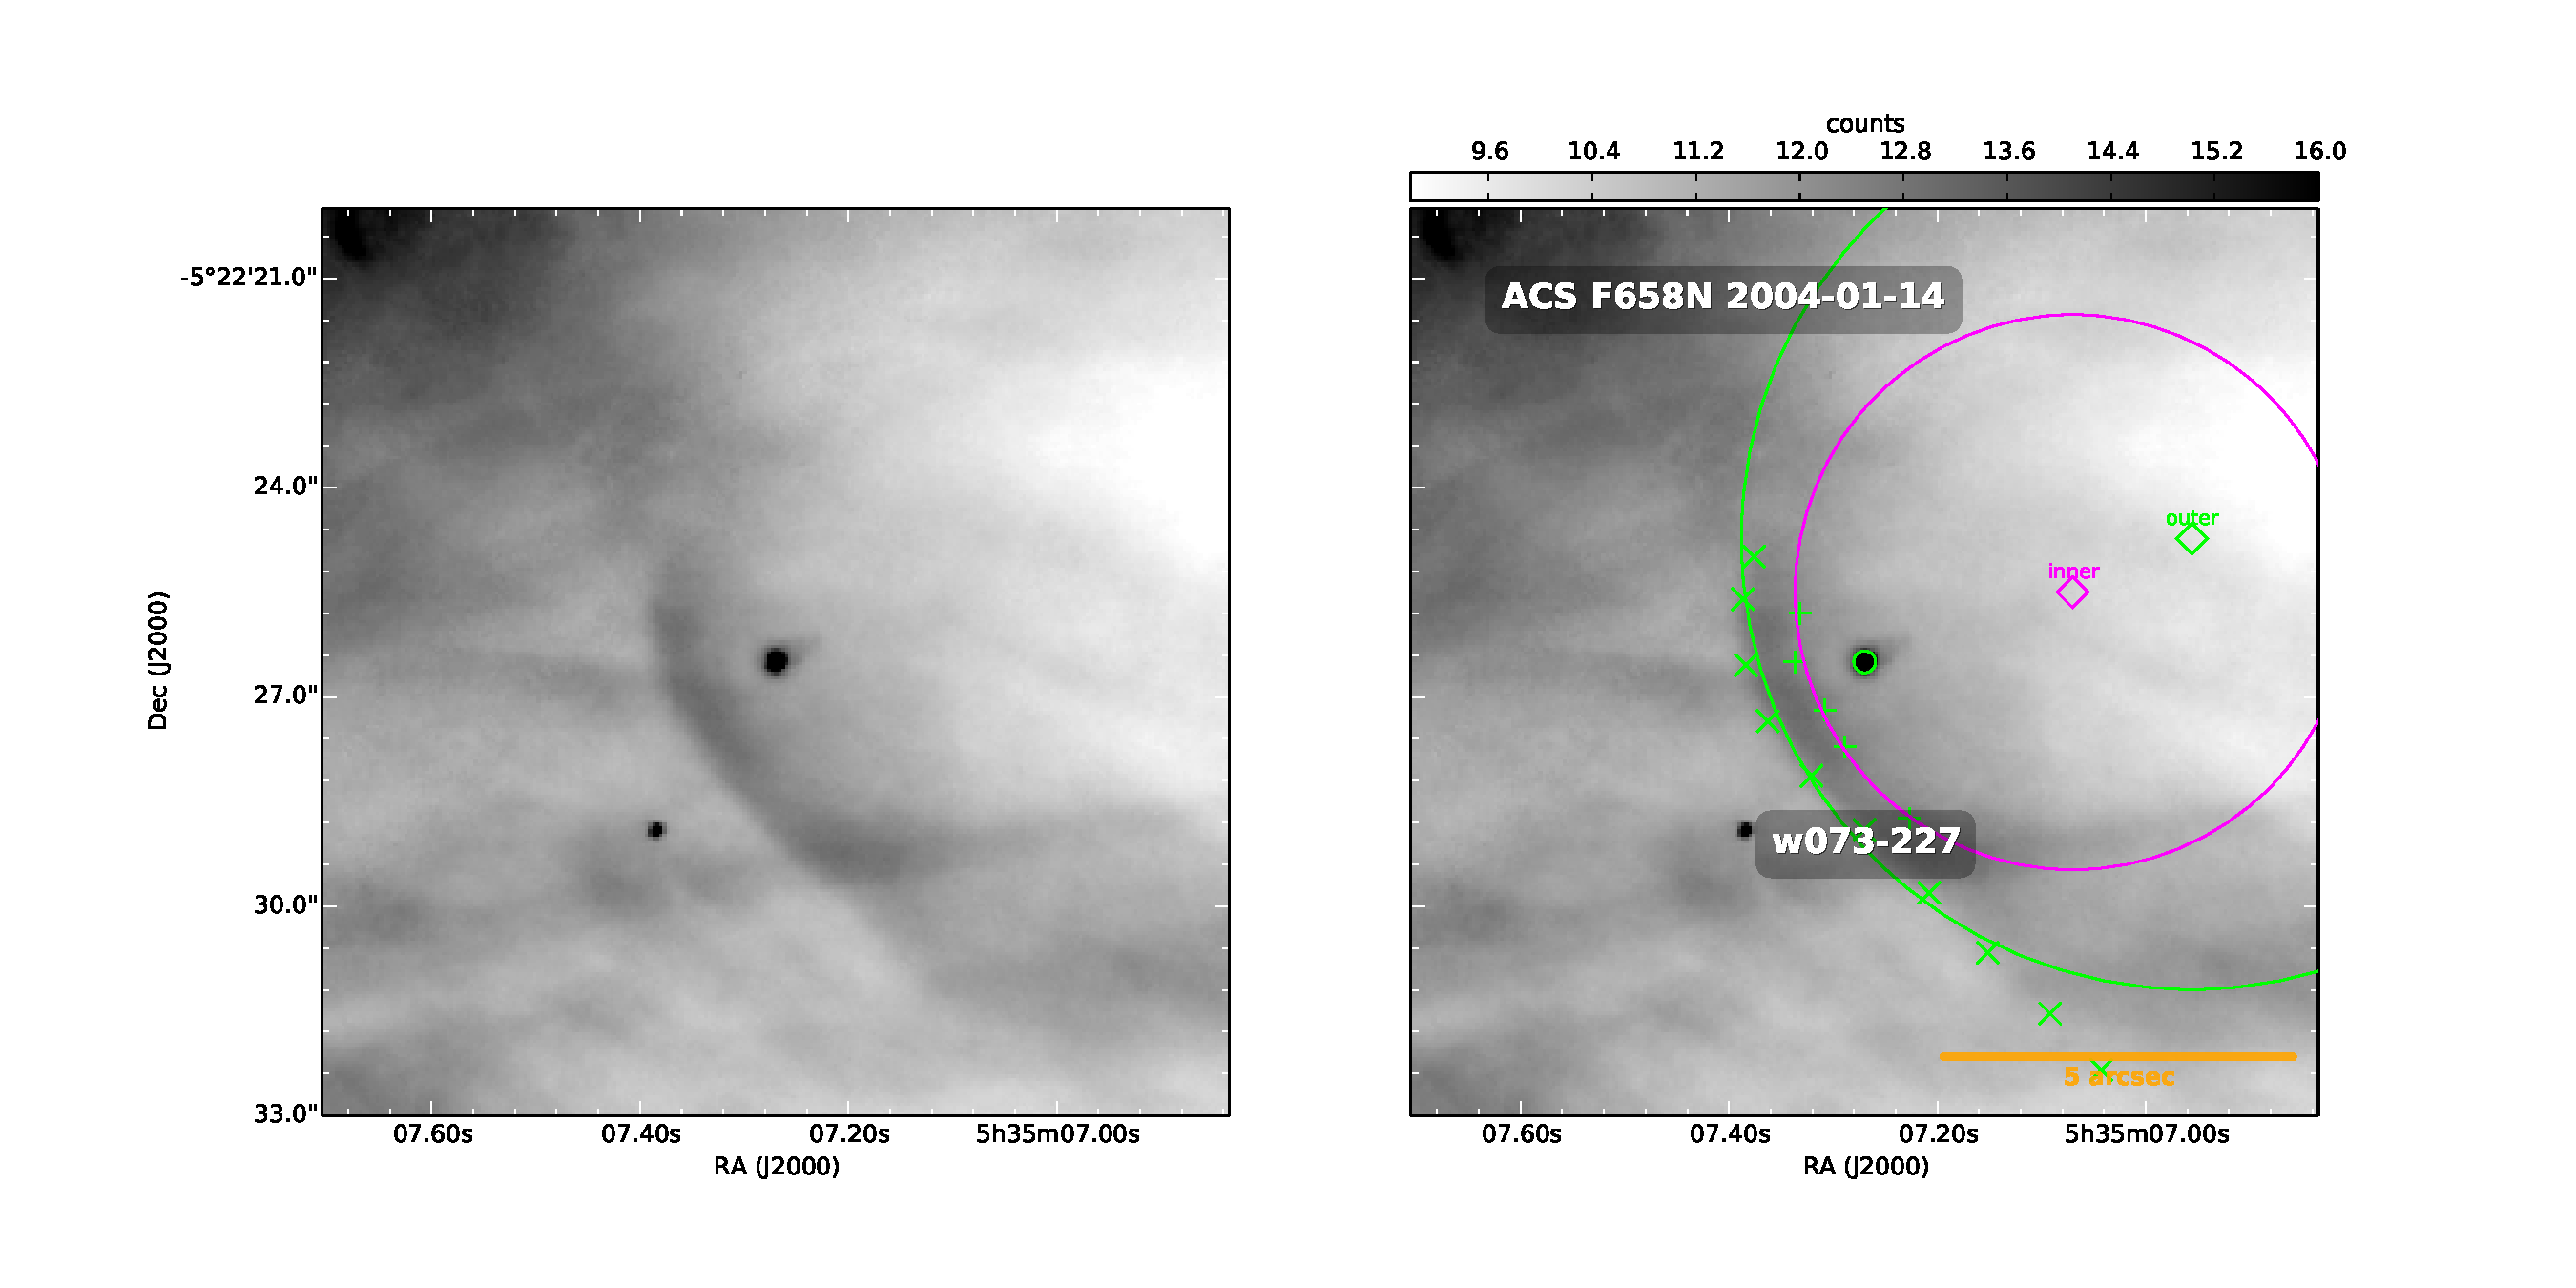
\includegraphics[width=0.95\linewidth, trim=60 20 60 60, clip]{./j8oc01010_wcs/w073-227-Bally_01-images.pdf}
\\
\end{tabular}
\caption{Forma de los arcos de (a) w069-601 y (b) w073-227.}\label{fig:forma}
\end{figure}

La forma de los arcos suelen diferir un poco puesto que estos  no son totalmente simétricos y como se logra apreciar en la figura \ref{fig:forma}, esto va a provocar que los círculos que se ajustan a dichos arcos tengan diferentes tamaños en cada uno de los objetos, esto es \(R_{c}\) un tanto distintos. Hay que decir que  w069-601 y w073-227 se encuentran en el campo 01 de las observaciones de Bally y deacuerdo al análisis realizado tienen por radios de curvatura 1.77 en el borde externo y 7.33 en el borde interno, esta corresponde a la imagen (a) de la figura~\ref{fig:forma} y 3.98 en el borde externo y 11.58 en el borde interno correspondiendo a la parte (b) de la figura \ref{fig:forma}. Si nos ubicamos en otro campo en las observaciones de Bally, por ejemplo en el campo 24 que tiene sólo a LL4 la forma del arco es como se observa en la fígura~\ref{fig:LL4} y es de notar que sus radios de curvatura son: 3.72 para el borde externo y 0.89 para el interno.\\

\begin{figure}
  \centering
  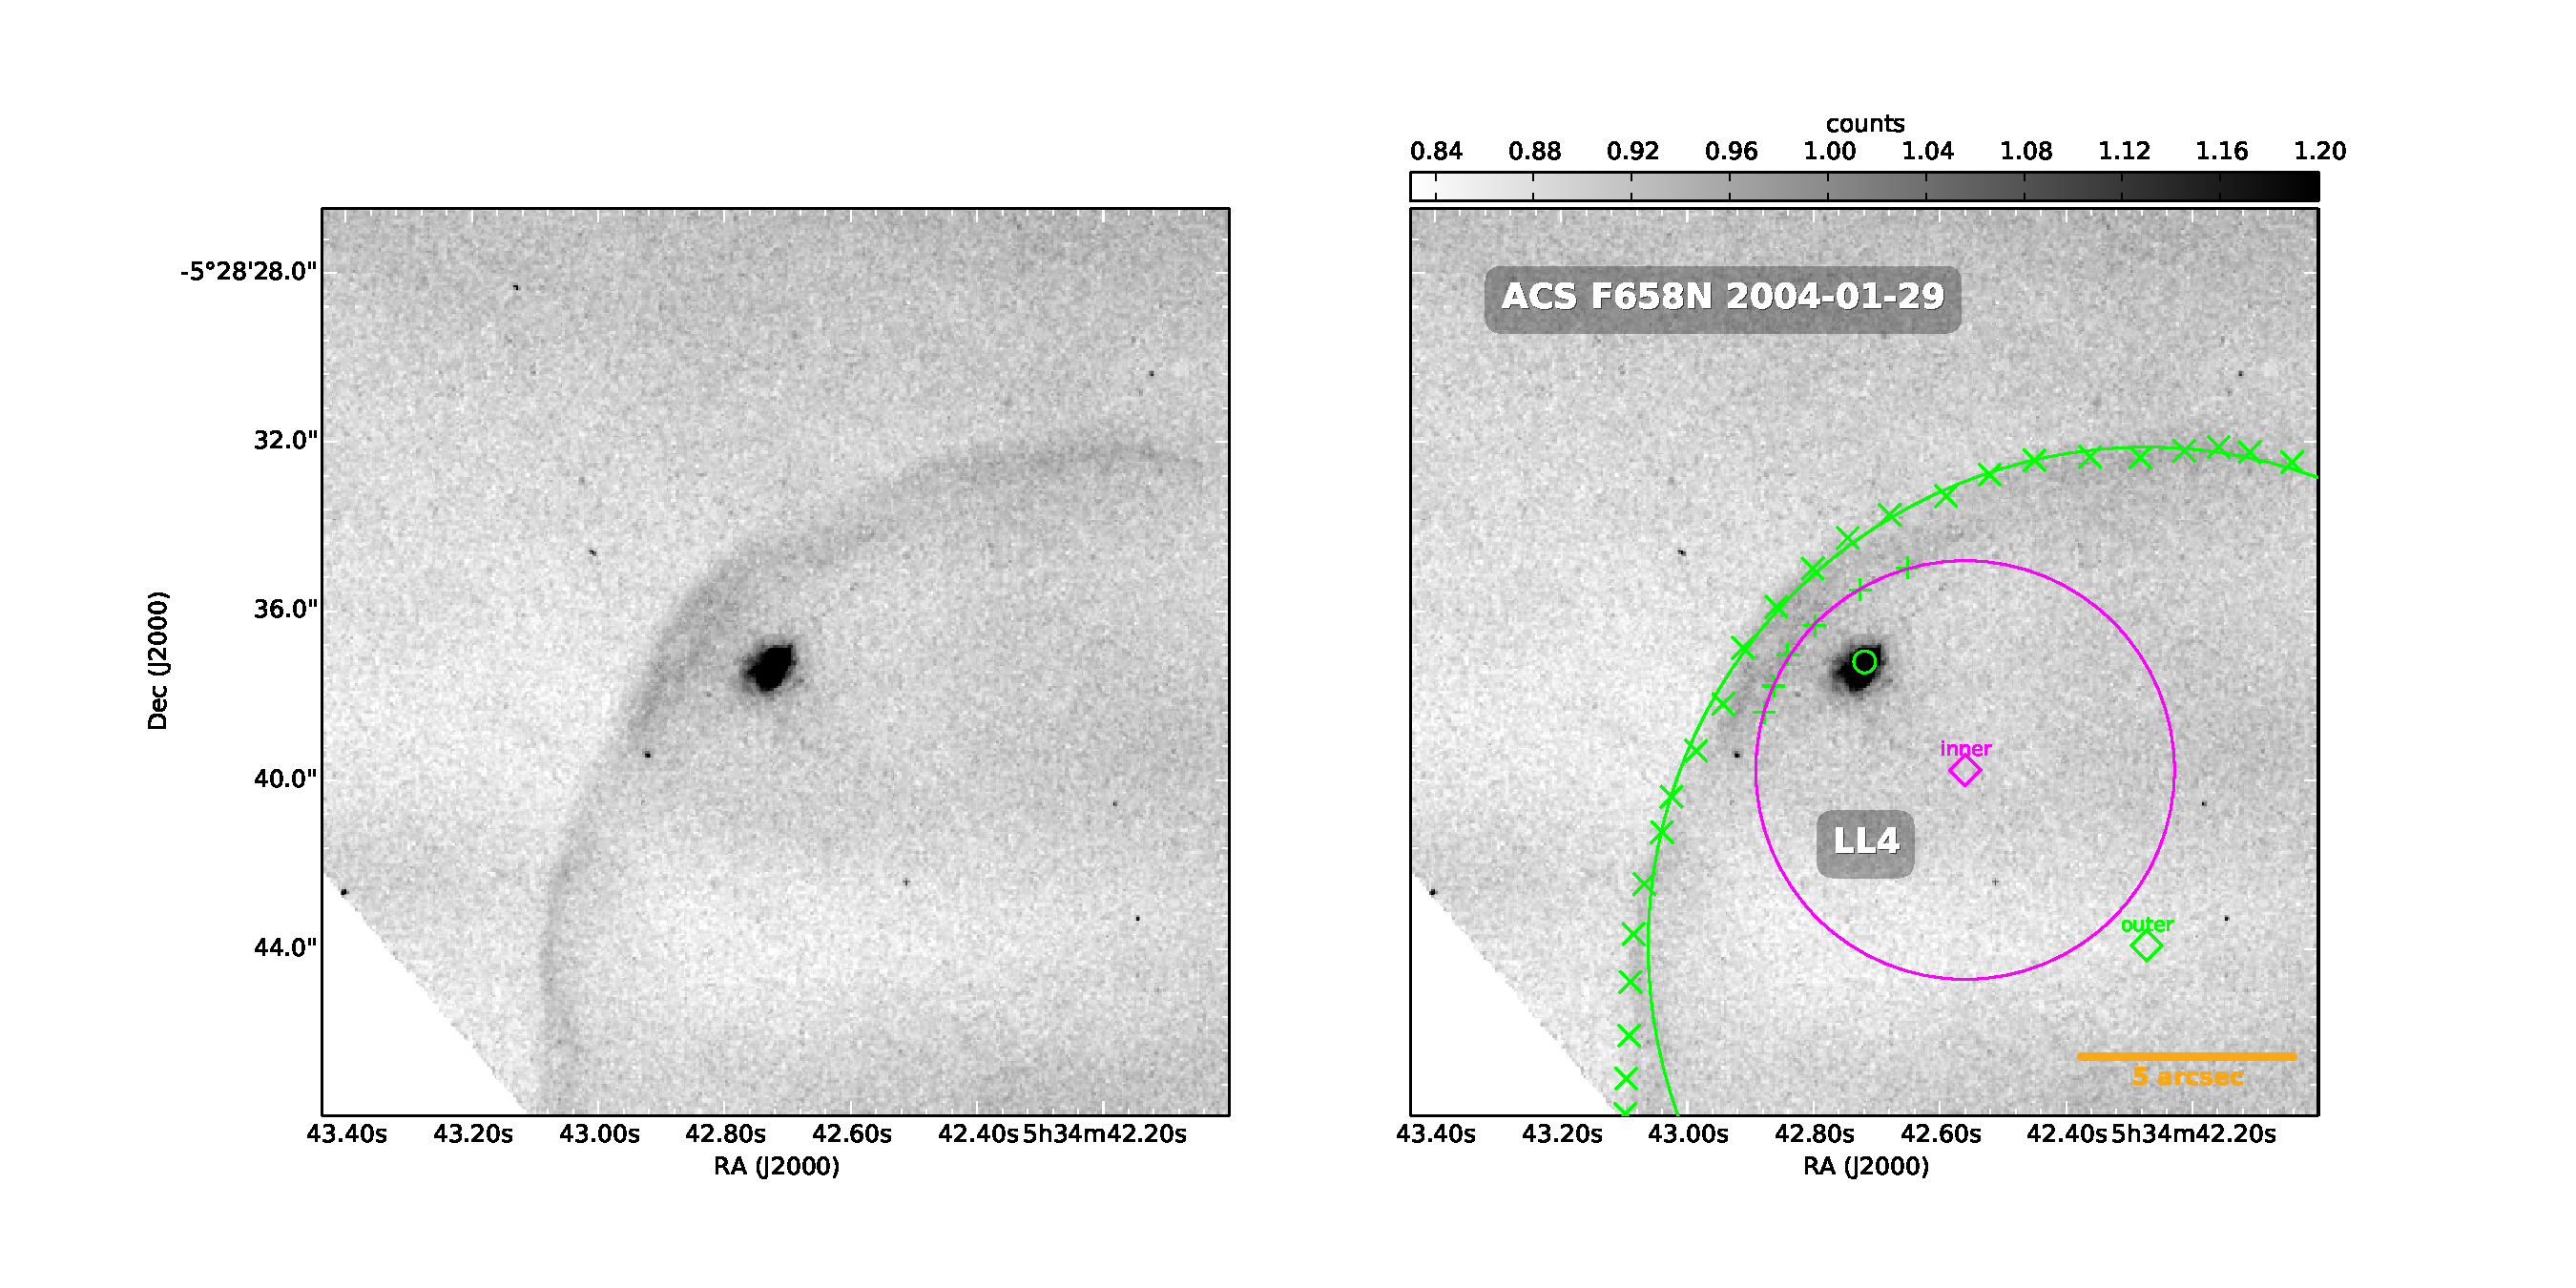
\includegraphics[width=\linewidth, trim=60 20 60 60, clip]{j8oc24010_wcs/LL4-Bally_24-images.pdf}
  \caption{Forma del arco de LL4.}
  \label{fig:LL4}
\end{figure}

\begin{figure}
  \centering
  \includegraphics[width=.45\linewidth, trim=30 20 30 20, clip]{j8oc01010_wcs/w012-407-Bally_01-arcbright-z.jpg}
  \includegraphics[width=.45\linewidth, trim=30 20 30 20, clip]{j8oc01010_wcs/w012-407-Bally_01-arcbright-th.jpg}
  \caption{Brillo superficial de LL1}
  \label{fig:brillo-LL1}
\end{figure}

De la misma manera como ya hemos trazado la región donde está el gas chocado, entonces se ha estimado el brillo superficial \(S_{\ha}\) en las diferentes zonas donde la estrella y el choque están estrechamente vinculadas, esto es en la cáscara y en el fondo. En este orden de ideas hemos podido graficar el brillo superficial en función de los ángulos de la cáscara externa, tomando como eje de simetría la dirección en que se encuentra la estrella masiva (ver figura \ref{fig:brillo-LL1}). Es importante señalar que hasta el momento hemos calculado los radio de curvatura \(R_{c}\), la distancia de los choques a la estrella \(R_{0}\) y hemos estimado el brillo superficial \(S_{\ha}\) de los 72 Objetos LL que se han agregado a la lista, subrayando que para ello hemos utilizado principalmente los campos de Bally. 


\bibliography{luis-ref}

\end{document}
